	% Predlozak za pisanje diplomskog rada na PMF-MO
% Opcenita uputstva za LaTeX se mogu npr. naci na 
% http://web.math.hr/nastava/rp3, http://web.math.hr/nastava/s4-prof/latex.pdf
% NE PREPORUCA se "Ne baš tako kratak uvod u TEX", buduci se radi o vrlo starom prirucniku
% koji nije pogodan za moderne verzije LaTEXa.
% Originalna verzija "The not so short..." na http://tobi.oetiker.ch/lshort/lshort.pdf 
% je obnovljena i daje bolji uvid u moderne verzije LaTeXa

% Stil je optimiziran za kreiranje pdf dokumenta (npr. pomocu pdflatex-a, XeLaTeX-a)

\documentclass[a4paper,oneside,12pt]{memoir} % jednostrano: promijeniti twoside u oneside

% Paket inputenc omogucava direktno unosenje hrvatskih dijakritickih znakova 
% opcija utf8 za unicode (unix, linux, mac)
% opcija cp1250 za windowse
\usepackage[utf8]{inputenc}  % ukoliko se koristi XeLaTeX onda je \usepackage{xunicode}\usepackage{xltxtra}
\usepackage{color}
% Stil za diplomski, unutra je ukljucena podrska za hrvatski jezik
\usepackage{diplomski}
% bibliografija na hrvatskom
\usepackage[languagenames,fixlanguage,croatian]{babelbib} % zahtijeva datoteku croatian.bdf
% hiperlinkovi 
\usepackage[pdftex]{hyperref} % ukoliko se koristi XeLaTeX onda je \usepackage[xetex]{hyperref}

\usepackage{listings}

\DisemulatePackage{setspace}
\usepackage{setspace}
\usepackage[]{algorithm2e}
% Odabir familije fontova:
% koristenjem XeLaTeX-a mogu se koristiti svi fontovi instalirani na racunalu, npr
% \defaultfontfeatures{Mapping=tex-text}
% \setmainfont[Ligatures={Common}]{Hoefler Text}
% ili
% \newcommand{\nas}[1]{\fontspec{Adobe Garamond Pro}\fontsize{24pt}{24pt}\color{Chocolate}\selectfont #1}
% i onda \nas{Naslov ...}
\usepackage{txfonts} % times new roman 
% Paket graphicx sluzi za manipuliranje grafikom 
\usepackage[pdftex]{graphicx} % ukoliko se koristi XeLaTeX onda je \usepackage[xetex]{graphicx}
% Paket amsmath je vec ukljucen
% Dodatno definirane matematicke okoline:
% teorem (okolina: thm), lema (okolina: lem), korolar (okolina: cor),
% propozicija (okolina: prop), definicija (okolina: defn), napomena (okolina: rem),
% slutnja (okolina: conj), primjer (okolina: exa), dokaz (okolina: proof)
% Definirane su naredbe za ispisivanje skupova N, Z, Q, R i C
% Definirane su naredbe za funkcije koje se u hrvatskoj notaciji oznacavaju drukcije 
% nego u americkoj: tg, ctg, ... (\tgh za tangens hiperbolni)
% Takodjer su definirane naredbe za Ker i Im (da bi se razlikovala od naredbe za imaginarni dio kompleksnog
% broja, naredba se zove \slika).

\pagestyle{headings}
% uz paket fancyhdr mogu se lako kreirati fancy zaglavlja i podnozja



% Podaci koje treba unijeti
\title{DNA kriptografija}
\author{Antonio Kovačić}
\advisor{prof. dr. sc. Andrej Dujella}  % obavezno s titulom (prof. dr. sc ili doc. dr. sc.)
\date{srpanj, 2014.}  % oblika mjesec, godina

% Moguce je unijeti i posvetu
% Ukoliko nema posvete, dovoljno je iskomentirati/izbrisati sljedeci redak 
\dedication{Ovaj diplomski rad posvećujem svojim roditeljima, sestri, braći, prijateljima, mentoru, profesorima, kolegama s faksa, kao i svim ljudima koji su doprinijeli kako mom intelektualnom rastu, tako i mom rastu kao cjelovite osobe.}

\begin{document}

% Naredna frontmatter generira naslovnu stranicu, stranicu za potpise povjerenstva, eventualnu posvetu i sadrzaj
% Moze se iskomentirati ukoliko nije u pitanju konacna verzija
\begin{spacing}{1.5}
\frontmatter

% Tekst diplomskog ...

% Diplomski rad treba poceti s uvodnim poglavljem  
\begin{intro}

U današnje vrijeme svjedoci smo nagloga porasta razmjene podataka. Naglim napretkom današnjih računala, javila se potreba za povećanjem sigurnosti, odnosno zaštite podataka, koji putuju preko komunikacijskog kanala. Današnji kriptosustavi omogućuju siguran prijenos takvih podataka, a ključ njihovog razbijanja zapravo leži u faktoriziranju nekog \textit{velikog} broja (na primjer \textsc{RSA} kriptosustav). Na današnjim računalima, takav problem nije lako riješiv - pa su ti sustavi još uvijek sigurni. Razvojem novih teoretskih modela računala - koji se pokušavaju i u praksi realizirati - uočeno je da problem faktorizacije neće biti više takav problem. Primjer jednog takvog računala je kvantno računalo za kojeg postoji algoritam (\textit{Shorov algoritam}) koji faktorizira broj u polinomnom vremenu.
Time se javila potreba za osmišljanjem  novih teoretskih modela računala - odnosno kriptosustava - koji bi bili otporni na kvantno izračunavanje - ne bi se mogli probiti uporabom kvantnog računala u nekom razumnom vremenu. Takve kriptosustave ćemo zvati \textit{kvantno rezistentnima}.
Tema ovog diplomskog rada biti će DNA kriptografija. Kratko rečeno, radi se o teoretskom modelu kriptografskog sustava koji pomoću DNA izračunavanja šifrira podatke. Prednost takvog sustava jest upravo što je kvantno rezistentan.\\[0.2cm]
U ovom radu najprije ćemo se ukratko upoznati s pojmom DNA računala, odnosno DNA izračunavanja, složenosti DNA računala te algoritmom za enkripciju, odnosno dekripciju podataka pomoću DNA računala.
\end{intro}
\chapter{DNA računalo}
\section{DNA izračunljivost}
\label{sec:DNAizr}
DNA stroj, kao ni DNA izračunavanje nećemo striktno definirati već će definicija biti opisna - u definiciji ćemo reći koje operacije DNA stroj može izvršavati, i što pri tome mora biti zadovoljeno.\\ Prije nego definiramo DNA stroj moramo definirati neke pojmove iz logike sudova i kombinatorike.
\begin{defn}
\textbf{Alfabet} je proizvoljan konačan skup, čije elemente nazivamo \textbf{simboli}.\\
Neka je $n \in \mathbb{N}$ proizvoljan te $A$ proizvoljan alfabet, proizvoljni element $w \in A^n$ zovemo \textbf{riječ alfabeta A}. Neka su $s_1,..., s_n \in A$, riječ $w=(s_1,...,s_n)$ alfabeta A još zapisujemo kao $w=s_1s_2...s_n$. Smatramo da postoji riječ alfabeta A, koju ćemo označavati s $\varepsilon$, koja se ne sastoji ni od jednog simbola i zovemo je \textbf{prazna riječ}. Po dogovoru smatramo da je $A^0=\{\varepsilon\}$. Skup svih riječi alfabeta $A$ označavamo sa $A^*$. Neka su $a=a_1...a_m$, te, $b=b_1...b_k \in A^*$, kažemo da je riječ $c \in A^*$ nastala \textbf{konkatenacijom} riječi $a$ i $b$ ako vrijedi $c=ab=a_1...a_mb_1...b_k$. Kažemo da je riječ $c \in A^*$ podriječ riječi $a \in A^*$, ako postoje riječi $b, d \in A^*$ tako da je $a=bcd$. \textbf{Duljina riječi} se definira kao funkcija $d:A^*\to \mathbb{N}$ sa:
\begin{align*}
	d(\varepsilon) :&= 0 \\
	d(wa) :&= d(w)+1
\end{align*}
\end{defn}
\begin{defn}
Neka je S proizvoljan konačan skup, a $m:S \to \mathbb{N}$ proizvoljna funkcija. \textbf{Multiskup M na skupu S} je uređeni par $M=(S,m)$. Za proizvoljan $x\in S$, $m(x)$ zovemo \textbf{kratnost} od $x$. \textbf{Kardinalnost multiskupa M} (broj elemenata), u oznaci $|M|$, se definira kao:
\[|M|:=\sum_{x \in S} m(x)\]
\end{defn}
\begin{defn}
 \textbf{DNA lanac} je proizvoljna riječ alfabeta \{A (adenin), G (gvanin), T(timin), C (citozin)\}. DNA stroj se sastoji od konstantnog broja konačnih skupova koje nazivamo \textbf{epruvete}, a čiji su elementi DNA lanci. Za proizvoljnu epruvetu K DNA stroja definiramo multiskup $MulS(K)$ kao multiskup svih riječi koje predstavljaju DNA lance sadržane u epruveti K. U DNA stroju su definirane slijedeće instrukcije:
    \begin{itemize}
        \item Kopiraj($K_1$,$K_2$) $\to$ uz pretpostavku da je $K_2$ = $\emptyset$ , kopira MulS($K_1$) u MulS($K_2$) time više $K_2$ nije prazan
        \item Spoji($K_1$, $K_2$, $K$) $\to$ uz pretpostavku da $K$=$\emptyset$: \[MulS(K)=MulS(K_1)\bigcup MulS(K_2) \]
        \item Uoči($K$) $\to$ ispituje je li $MulS(K)\neq\emptyset$, ako je rezultat operacije je $\top$, inače $\bot$. Također se može pročitati sadržaj epruvete $MulS(K)$.
        \item Odvoji(K,w) $\to$ za skup $K$ i riječ $w$ (iz $MulS(K)$) izbacuje sve riječi iz $K$ koje kao podriječ ne sadrže riječ $w$
        \item Izvadi(K,w) $\to$ $K\backslash Odvoji(K,w)\to $izbacuje sve riječi iz $K$ koje sadrže $w$
        \item Odvoji\textunderscore Pref(K,w) $\to$ izbacuje sve riječi iz K koje ne sadrže w kao prefiks
        \item Odvoji\textunderscore Suff(K,w) $\to$ izbacuje sve riječi iz K koje ne sadrže w kao sufiks
        \item Proširi(K) $\to$ multiskupu MulS(K) još jednom dodaje elemente od K
        \item Izdvoji\textunderscore po\textunderscore duljini(K, l) $\to$ iz K izbacuje sve riječi čija je duljina različita od l
        \item Konkatenacija(K) $\to$ na slučajan način izvodi operaciju konkatenacije nad riječima iz MulS(K) tako da duljina novonastalih riječi ne bude veća od neke konstante, a vraća multiskup koji sadrži sve riječi nastale tom konkatenacijom. Vjerojatnost nastajanja duljih riječi je veća. Ukoliko MulS(K) prije izvođenja ove operacije nad epruvetom K sadrži veliki broj kopija svake od riječi, tada će MulS(K) nakon izvođenja ove operacije nad epruvetom K sadržavati sve moguće kombinacije elemenata iz K.
            \begin{itemize}
                \item \textbf{Biološki komplement} DNA lanca H definiramo kao DNA lanac koja ima jednako znakova kao i H, ali je svaki znak A zamijenjen znakom T, a svaki znak C znakom G i obratno, i označavamo je s $\overline{H}$
                \item Neka riječ H ima duljinu $n \in 2\mathbb{N}$, tada definiramo \textbf{biološki prefiks} riječi H kao biološki komplement riječi sastavljene od prvih $\frac{n}{2}$ znakova iz H, slično definiramo i \textbf{biološki sufiks} riječi H kao biološki komplement riječi sastavljene od zadnjih $\frac{n}{2}$ znakova riječi H
                \item Smatramo da je operacija konkatenacije nad riječima H i J dopuštena ako postoji riječ L takva da je biološki sufiks od H prvih $\frac{n}{2}$  znakova od L, a biološki prefiks od J prvih $\frac{n}{2}$ znakova od L
            \end{itemize}
    \item Izreži(K) $\to$ na slučajan način “skraćuje” riječi iz MulS(K) do neke fiksne duljine
    \item Izaberi(K) $\to$ na slučajan način iz MulS(K) izabire neku riječ te “generira” novi skup sastavljen od samo te riječi

    \end{itemize}
    \textbf{Program za DNA stroj} definiramo kao konačan niz gornje navedenih instrukcija. U svakom koraku programa se može izvesti točno jedna instrukcija.  Kažemo da program P za DNA stroj \textbf{izračunava} funkciju $f:S \subseteq N^k \to \N$ ako vrijedi:\\
$\vec{x}=(x_1,...,x_k) \in S$ ako i samo ako program P za DNA stroj s ulazom  $\vec{x}$ (reprezentiranim pomoću DNA lanaca) u epruveti K završi s izvršavanjem te na kraju izvršavanja vrijedi \textit{Uoči(K)}$=\top$ te je pri tome $K=\{f(\vec{x})\}$.\\
Kažemo da je funkcija $f:\N \to \N$ \textbf{DNA izračunljiva} ako postoji program za DNA stroj koji ju izračunava.
\end{defn}
\begin{rem}
Vidimo da se sve ove operacije izvršavaju nad jednom epruvetom u jednom koraku, odnosno multiskupom $MulS(K)$. Što je veća kardinalnost multiskupa $MulS(K)$, to se više operacija na riječima izvrši istovremeno, a u stvarnom svijetu sve te operacije imaju svoje "biokemijske analogone" - biokemijske reakcije. Takvo računalo zapravo možemo interpretirati kao superračunalo s izuzetno velikim brojem procesora. U pozadini svega toga se zapravo krije masivni paralelizam. Memoriju DNA računala zapravo predstavljaju epruvete. Jasno je odakle naziv epruvete.\\
Uočimoo da je $MulS(K)$ definiran nad konačnim skupom pa je i on konačan - no vidimo da se on zapravo može proširiti nizom operacija \textit{Proširi} tako da je njegov kardinalitet izrazito velikog reda (nadeksponencijalnog) , ali u praksi se već sada zaključuje da to neće biti uvijek moguće - naime broj DNA lanaca u epruveti (laboratorijskoj) biti će ograničen volumenom te epruvete.\\
Uočimo da operacija konkatenacije uključuje vjerojatnosni efekt - \textit{vjerojatnost nastajanja duljih riječi konkatenacijom je veća} - odnosno dvije riječi iz skupa $K$ koje će se konkatenirati neće biti izabrane na slučajan način - već tako da se pokuša dobiti riječ maksimalne duljine (maksimalna duljina je određena nekom konstantom). Iz toga očito možemo vidjeti da sam ishod DNA računanja nije sasvim siguran  - no u praksi se pokazuje (pri sintezi DNA lanaca) da je to moguće - u tu svrhu je i uvedena pretpostavka da će  se, ukoliko $MulS(K)$ sadrži velik broj kopija od svake riječi iz $K$, dobiti svaka moguća konkatenacija riječi iz $K$.
\end{rem}
\section{O složenosti DNA računala}
Kako bi nešto rekli o složenosti DNA računala, najprije ćemo navesti nekoliko osnovnih definicija iz teorije složenosti algoritama, odnosno referencirati se na \cite{Sipser}.
\begin{defn}
\textbf{Turingov stroj} je uređena sedmorka $(Q, \Sigma , \Gamma , \delta, q_0, q_{DA}, q_{NE})$, gdje je redom:
\begin{itemize}
	\item Q konačan skup čije elemente nazivamo stanja
	\item $\Sigma$ je konačan skup, čije elemente nazivamo ulazni simboli, pretpostavljamo da $\Sigma$ ne sadrži "prazan simbol" kojeg označavamo sa $\varepsilon$
	\item $\Gamma$ je konačan skup kojeg nazivamo alfabet Turingovog stroja, pretpostavljamo da je $\varepsilon \in \Gamma$, te $\Sigma \subset \Gamma$
	\item $\delta : Q \times \Gamma \to Q \times \Gamma \times \{ L,D,S\}$ koju nazivamo funkcija prijelaza
	\item $q_0 \in Q$ nazivamo početnim stanjem
	\item  $q_{DA} \in Q$ nazivamo stanjem prihvaćanja
	\item $q_{NE} \in Q$ nazivamo stanjem odbijanja, te $q_{NE}\neq q_{DA}$
\end{itemize}
\end{defn}
\begin{rem} (Opis rada Turingovog stroja)\\
Turingov stroj zapravo ima četiri glavna dijela: kontrolnu jedinicu (koja zapravo oponaša dijelovanje funkcije $\delta$), beskonačnu traku, neograničenu s lijeve i desne strane, takvu da se u svakom trenutku rada stroja na jednom registru trake nalazi točno jedan simbol, memoriju u kojoj se pamti trenutačno stanje stroja te glavu za čitanje koja se u jednom koraku rada stroja može pomicati za točno jedno mjesto na traci: desno, lijevo ili ostati na istom simbolu. Glava se na početku nalazi na nekom mjestu na traci (unaprijed definiranom), zatim čita simbol. Pročitani simbol, u paru s trenutnim stanjem stroja "se šalje" u kontrolnu jedinicu. Glava nakon toga, najprije zamijeni pročitani simbol nekim drugim simbolom, stroj prelazi u novo stanje, a glava se pomiče na drugi registar (L (lijevo), D (desno)) ili ostaje na istom mjestu (S). \\
Vidimo da opisani Turingov stroj može stati u dva završna stanja $q_{DA}$, odnosno $q_{NE}$, takav Turingov stroj se naziva još odlučitelj. Uočimo da Turingov stroj ne mora nužno uvijek stati. Shematski prikaz Turingovog stroja možete vidjeti na slici \ref{fig:Turing}.\\
Nedeterministički Turingov stroj se definira na analogan način, samo što je funkcija prijelaza definirana sa: $\delta : Q \times \Gamma \to \mathcal{P}(Q \times \Gamma \times \{L,D,S\})$. 
\end{rem}
\begin{figure}[h!t]
\centering 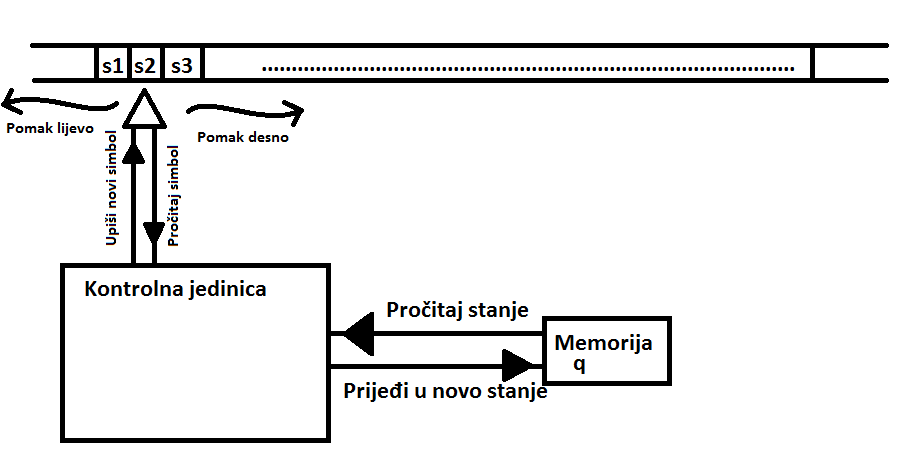
\includegraphics[height=200pt, width=400pt]{Turing.png}
\caption{Shematski prikaz Turingovog stroja}
\label{fig:Turing}
\end{figure} 
\begin{defn}
Neka su $f, g: \N \to \R^{+}$ dvije funkcije. Kažemo da je funkcija $g$ \textbf{asimptotska gornja međa} za funkciju $f$ ako postoje $c>0$ i $n_0 \in \N$ tako da za svaki $n \geq n_0$ vrijedi
\[f(n)\leq cg(n)\]
Činjenicu da je $g$ asimptotska međa od $f$ označavamo sa $f(n)=O(g(n)$. 
\end{defn}
Osnovne definicije (što je alfabet logike sudova, interpretacija, ispunjivost formule, konjunktivna, odnosno, disjunktivna normalna forma  i tako dalje) se mogu naći u \cite[s. ~12-25]{Vukovic}.\\
Više o Turingovom stroju te nekim pojmovima na koje se pozivamo u idućim rezultatima se mogu naći u:
\begin{itemize}
\item Turing prepoznatiljivost, Turing odlučivost \cite[s. ~141-142]{Sipser}
\item Vremenska složenost Turingovog stroja determinističkog se može naći u \cite[s. ~248]{Sipser}, a nedeterminističkog u \cite[s. ~255]{Sipser}
\item Klase vremenske složenosti:
 \begin{itemize}
 	\item $TIME(f(n))$ u \cite[s. ~251]{Sipser}
 	\item $P$  u \cite[s. ~258]{Sipser}
 	\item Vezano uz klasu $NP$ u \cite[s. ~265-267]{Sipser}
 \end{itemize}
 
 	\item Polinomna reducibilnost u \cite[s. ~272]{Sipser}
 	\item NP-potpunost u \cite[s. ~276]{Sipser}
\end{itemize}
Označimo sa $SAT$ skup definiran na idući način:
\[SAT=\{F: F \textrm{ je ispunjiva formula logike sudova }\}\]
Formulacija \textit{problema SAT} glasi:\\
\begin{center}
Za danu formulu logike sudova F koja je u konjunktivnoj normalnoj formi odrediti\\ vrijedi li $F \in  SAT$.
\end{center}
Konjunktivnu normalnu formu koja u svakoj svojoj elementarnoj disjunkciji sadrži točno $k \in \N \backslash \{0\}$ literala nazivamo $k$-knf. Formulacija problema $k-SAT$ glasi:
\begin{center}
	Za proizvoljnu formulu $F$ koja je $k$-knf odrediti je li $F$ ispunjiva. 
\end{center} 
U \cite[s. ~276-283]{Sipser} se može vidjeti da je problem $SAT$ \textit{NP-potpun} problem, kao i $3-SAT$.
Sljedeći teorem govori zapravo o tome da DNA računala, u pogledu vremenske složenosti, imaju bolja svojstva nego deterministički Turnigovi strojevi:
\begin{thm} (Lipton)
Za svaku konjunktivnu normalnu formu $F$ u kojoj se pojavljuje $n$ propozicionalih varijabli i $m$ klauzula, u $\mathcal{O}(m+1)$ separacija i $\mathcal{O}(m)$ spajanja te jednim uočavanjem možemo odlučiti vrijedi li $F \in SAT$
\end{thm}
Dokaz navedenog teorema se može naći u \cite{Lipton}.\\
S pogleda odlučivosti jezika ipak nemamo takav rezultat, odnosno postoji slutnja koja kaže:
\begin{conj} (Kvantna i biološka slutnja) Problem je odlučiv na DNA računalu ili kvantnom računalu ako i samo ako je Turing-odlučiv.
\end{conj}
Postavlja se prirodno pitanje kako izračunati složenost DNA računala. Odgovor je jednostavan: složenost DNA računala procijenjujemo brojem instrukcija koje DNA stroj izvrši, te s kardinalosti skupa $MulS(K)$. Zbog toga što kardinalnost skupa $MulS(K)$ može izrazito brzo rasti (samo jedna operacija \textit{Proširi(K)}, za pripadnu funkciju kratnosti $m$ multiskupa $MulS(K)$ vrijedi da je: $m_{nova}(x)=2\cdot m_{stara}(x)$, gdje je $m_{nova}(x)$ kratnost od $x$ nakon izvršenja operacije \textit{Proširi},a $m_{stara}(x)$ kratnost od $x$ prije izvršenja te iste operacije) prostorna složenost nekog programa za DNA stroj obično doseže nadeksponencijalnu veličinu (vidjet ćemo u idućem podpoglavlju takav slučaj). \\
U sljedećem potpoglavlju ćemo procijeniti složenost jednog programa za DNA stroj.
\subsection{Problem Hamiltonovog puta}
\begin{defn}
\textbf{Konačan usmjereni graf} je uređeni par $G=(V,E)$ gdje je V proizvoljan konačan skup čije elemente nazivamo \textbf{vrhovi}, a $E\subseteq V \times V$ skup čije elemente nazivamo \textbf{bridovi}. Ako je $E=V\times	V$ kažemo da je usmjereni graf $G$ \textbf{potpuni graf}. Kažemo da je brid $e$ \textbf{petlja} ako vrijedi:
$(\exists x \in V) : e=(x,x)$.
\textbf{Šetnja u grafu} G je $2n+1$-torka $(v_0,e_0,v_1,e_1,...,v_{n-1},e_{n-1}, v_{n})$, pri čemu vrijedi:
\begin{itemize}
	\item $(\forall i \in \{0,...,n\}) \quad v_i \in V$
	\item $(\forall i \in \{0,...,n-1\}) \quad e_i \in E$
	\item $e_i=(v_i, v_{i+1}), \forall i \in \{0,...,n-1\}$
\end{itemize}
Kažemo da šetnja  $(v_0,e_0,v_1,e_1,...,v_{n-1},e_{n-1}, v_{n})$ \textbf{prolazi kroz vrh} $x \in V$ ako postoji $i \in \{0,...,n\}$ takav da je $x=v_i$, te da šetnja \textbf{počinje} s vrhom $v_0$ i \textbf{zavšrava} s vrhom $v_n$. Duljina šetnje se definira kao broj bridova koji se pojavljuju u njoj.\\
\textbf{Staza} u grafu je šetnja $(v_0,e_0,v_1,e_1,...,v_{n-1},e_{n-1}, v_{n})$ za koju vrijedi 
\[(\forall i,j \in \{0,...,n-1\})\, (i\neq j) \to e_i \neq e_j\] \textbf{Put} u grafu je šetnja $(v_0,e_0,v_1,e_1,...,v_{n-1},e_{n-1}, v_{n})$ za koju vrijedi:
\[(\forall i,j \in \{0,...,n\})\, (i\neq j) \to v_i \neq v_j\] \textbf{Hamiltonov put} je put koji prolazi kroz sve vrhove grafa G.
\end{defn}
\begin{rem}
Neusmjereni graf se definira analogno, ali se skup bridova definira kao:
\[E\subseteq \{\{x,y\} : x, y \in V\}\]
Također, radi jednostavnosti, pretpostavili smo da između dva vrha $x,y \in V$ može biti najviše dva usmjerena brida i u tom slučaju vrijedi: $(x,y) \in E$ i $(y,x) \in E$.  
\end{rem}
Problem Hamiltonovog puta glasi:\\
\begin{center}
\textit{Postoji li u proizvoljnom konačnom grafu $G=(V,E)$ za vrhove $x,y \in V$  Hamiltonov put koji počinje s $x$, a završava s $y$.}
\end{center}
U \cite[s. ~286-291]{Sipser} se može vidjeti da je problem Hamiltonovog puta NP-potpun problem. U ovom poglavlju analiziramo \textit{Adlemanov algoritam} koji riješava problem u $\mathcal{O}(n \log (n))$ operacija. U kasnijim poglavljima ćemo obrazložiti reprezentaciju podataka pomoću DNA lanaca, za sada ćemo samo reći da su naši podaci reprezentirani lancima parne duljine $l$. Sada ćemo prezentirat Adlemanov algoriatam za traženje Hamiltonovog puta koji počinje s vrhom $v_{in}$, a završava s $v_{out}$ u usmjerenom označenom grafu $G=(V,E)$. Ali prije toga ćemo reći nešto o vezi bridova i vrhova. Ako su dani vrhovi $A$ i $B$ i reprezentirani riječima $H$ i $J$, tada je brid $(A,B)$ reprezentiran riječju koja je nastala konkatenacijom (u smislu operacije nad riječima) biološkog sufiksa riječi $H$ i biološkog prefiksa riječi $J$. Kako bi mogli razlikovati koji brid povezuje koje vrhove, uviđamo da svaki vrh mora imati jedinstveni prefiks i sufiks, a ne samo jedinstven prikaz jednom riječju. 
    Nakon što smo objasnili vezu između bridova i vrhova moramo najprije "pripremiti" epruvetu za algoritam. \[K=V\cup E\]
    U početku je upravo $MulS(K)=K$.\\
    \indent Adlemanov algoritam:
    \begin{enumerate}
        \item Ulaz: Graf $G=(V,E)$, $|V|=n$, $v_1=v_{in}$ vrh iz kojeg krećemo, $v_n=v_{out}$ vrh u kojem završavamo, stavi vrhove i bridove u $K$
        \item $ \lceil 2n\log_{2}(n) \rceil$ puta primjeni operaciju \textit{Proširi(K)} tako da dobiješ barem $2^{2n\log_{2}(n)}=n^{2n}$ kopija svake riječi u $MulS(K)$
        \item Primjeni operaciju \textit{Konkatenacija(K)} da dobiješ šetnju u $G$, tako da duljina šetnje bude manja od $n$ - broj bridova u šetnji može biti manji ili jednak $n$
        \item Primjeni \textit{Odvoji\textunderscore Pref(K, $v_{in}$)}: izbacujemo one šetnje koje ne počinju vrhom $v_{in}$
        \item  \textit{Odvoji\textunderscore Suff(K, $v_{out}$)} : izbacujemo one šetnje koje ne završavaju s $v_{out}$
        \item Primjeni operaciju \textit{Izdvoji\textunderscore po \textunderscore duljini(K, $l\cdot n + l\cdot (n-1) $)} da iz $K (MulS(K))$ izbaciš sve one riječi koje u sebi ne sadrže točno $n$ vrhova i $n-1$ bridova (šetnje čija je duljina točno $n-1$)
        \item na $v_i$ primjeni operaciju \textit{Odvoji(K, $v_i$)} , $\forall{i} \in \{2,3,...,n-1\}$: iz $MulS(K)$ ukloni sve one šetnje u kojima se neki od vrhova ne pojavljuje
        \item \textit{Uoči(K)}: postoji li Hamiltonov put
    \end{enumerate}


Nama zapravo bridovi u ovom algoritmu, na ovaj način konstruirani daju mogućnost povezivanja dva vrha koja su povezana nekim birdom (u smislu biokemije, igraju ulogu enzima inače se vrhovi ne bi mogli povezati). \\
Brojimo korake algoritma:
\begin{itemize}
\item 2: $\lceil 2n \log _2 (n) \rceil$ koraka
\item  3-6: Po jedan korak svaka operacija
\item 7: $n-2$ koraka
\item 8: jedan korak
\end{itemize}
Ukupno: $\lceil 2n \log _2 (n) \rceil + n-2 + 5=\lceil 2n \log _2 (n) \rceil + n+3 = \mathcal{O}(n \log(n))$ operacija. No, rekli smo da se složenost DNA stroja mjeri i kardinalnošću skupa $MulS(K)$ koji u jednom trenutku sadrži i $n^{2n}$ elemenata. 
Još je preostalo dokazati da algoritam radi:
\begin{thm} Neka je G=(V,E) usmjeren označen graf, te $v_{in}$ i $v_{out}$ elementi iz V, tada Adlemanov algoritam odlučuje postoji li u usmjerenom grafu G=(V,E) Hamiltonov put od $v_{in}$ do $v_{out}$. \end{thm}

\begin{proof}
    \begin{itemize}
        \item $|V|=n$, $K=V\cup E$ gdje smatramo da je svakom vrhu dodijeljen jedinstven prefiks i sufiks. Neka je minimalni DNA lanac duljine $l$.
        \item Definiramo rekurzivno skupove $MulS(K_n)$ odakle ćemo zapravo izvući kako izgleda naš skup $MulS(K)$ nakon primjene operacije \textit{Proširi(K)} $\lceil 2n\log_2(n) \rceil$ puta
        \[K_0=K \to MulS(K_0)=K_0\]
        \[MulS(K_{n+1})=MulS(K_n) \cup MulS(K_n) , n \in \mathbb{N}\]
        Nakon ovog koraka, redefiniramo skup MulS(K)
        \[MulS(K)=MulS(K_{\lceil 2n\log_2(n) \rceil})\]
        Zapravo sada trebamo dokazati da je $2^{\lceil 2n\log_2(n) \rceil}$ dovoljan broj kopija skupa K za kreiranje svih šetnji u grafu:
        \[2^{\lceil 2n\log_2(n) \rceil} \geq 2^{ 2n\log_2(n) } = n^{2n}\]
        pa je dovoljno pokazati da je $n^{2n}$ dovoljan broj kopija skupa K od kojih možemo kreirati sve šetnje u grafu. Bez smanjenja općenitosti u tu svrhu možemo pretpostaviti da je G potpuno povezan usmjeren graf (dakle svaki brid je povezan sa svakim u oba smjera). Zašto? Jer ako G nije potpuno povezan onda ima manji broj šetnji od potpuno povezanog usmjerenog grafa. \\
        \noindent U tu svrhu definiramo skup $A^k$:
        \[A^k=\{(b_1,...,b_k): b_i \in V\}\]
        Uvidimo da smo u skupu $A^k$ dozvolili i petlje! Dakle može postojati brid $(v_i, v_i)$. Kada to ne bi dozvolili, na uređenu $k$-torku bi samo još stavili uvjet da je $b_i \neq b_{i+1}, \quad \forall i \in \{1,...,k-1\}$.
        Sada, jer između svaka 2 vrha ima točno 1 brid za svaki smjer koji povezuje te vrhove, vidimo da su sve šetnje duljine $k-1$ jedinstveno određene skupom $A^k$. Pa su sve šetnje do duljine $n-1$ (jer ćemo tako izabrati operaciju konkatenacije da kreira šetnje duljine ne duže od $n-1$) reprezentirane idućim skupom:
        \[\bigcup_{k=1}^n A^k\]
        Preostalo je dokazati da kardinalnost gornjeg skupa nije veća od $n^{2n}$. Kardinalnost skupa $A^k$ je lako odrediti. Naime za prvu komponentu uređene $k$-torke ima $n$ mogućnosti, za $2$ isto $n$, općenito za $i$-tu komponentu ima $n$ mogućnosti.
        \[|A^k|=n^k \to \bigg|\bigcup_{k=1}^n A^k\bigg|=\sum_{k=1}^n |A^k|=\sum_{k=1}^n n^k=\frac{n(n^n-1)}{n-1}\]
        \[\frac{n(n^n-1)}{n-1} \leq \frac{n\cdot n^n}{n-1} \leq n\cdot n^n =n^{n+1} \leq n^{2n}\]
        \item Primjenom operacije \textit{Konkatenacija(K)} dobili smo sve moguće šetnje u grafu $G$ (spremljene u $MulS(K)$)
        \item Operacijama \textit{Odvoji\textunderscore Pref(K, $v_{in}$)} i \textit{Odvoji\textunderscore Suff(K, $v_{out}$)} iz skupa $MulS(K)$ izbacujemo sve one šetnje koje ne počinju vrhovima $v_{in}$ i $v_{out}$
        \item operacijom \textit{Izdvoji\textunderscore po\textunderscore duljini(K, $l\cdot n + l\cdot (n-1)$)} uklanjamo sve preostale bridove i one šetnje čija je duljina strogo manja od $n-1$.
        Sada su ostale šetnje duljine $n-1$, ali to još nisu putevi (a onda ni Hamiltonovi putevi). Kako ima $n$ vrhova, a šetnja je duljine $n-1$, to znači da je u šetnji točno $n$ vrhova kroz koje šetnja prolazi, ako se neki vrh ne nalazi u šetnji, to znači da se neki drugi vrh pojavljuje dva puta. A kako smo već uklonili one šetnje koje ne počinju s  $v_{in}$ i ne završavaju s $v_{out}$ jedino je preostalo ukloniti sve one šetnje koje ne sadrže neki $v_i \in V \backslash \{v_{in}, v_{out}\}$.
        \item Za svaki $x \in V \backslash \{v_{in}, v_{out}\}$ čini:
        \[Odvoji(K,x)\]
        \item Ovim su korakom zapravo u $MulS(K)$ ostali samo Hamiltonovi putevi koji počinju s  $v_{in}$ i završavaju s $v_{out}$, ako takvih ima, operacijom \textit{Uoči(K)} dobivamo rješenje.
    \end{itemize} 
\end{proof}
\chapter{DNA kriptografija}
\section{Osnovni biološki koncepti deoksiribonukleinske kiseline}
\label{sec:DNA}
\textbf{Deoksiribonukleinska kiselina} (DNA) sastavljena je od dva duga lanca nukleotida (polinukleotidni lanci) koji su omotani jedan oko drugoga, odnosno ima strukturu \textit{dvostruke uzvojnice }(engleski \textbf{double helix}) (slika \ref{fig:DNA}). \textbf{Nukleotid} je osnovna građevna jedinica DNA, a gradi ju jedna od četiri dušićne baze: \textit{adenina (A), gvanina (G), timina (T) i citozina (C)}, šećera pentoze te fosfatne skupine. Sa $1' - 5'$ označavamo ugljikove atome u molekuli šećera, a na slici \ref{fig:Nukleotid} se može vidjeti atomska struktura nukleotida. Vidimo da ako se na $2'$ veže hidroksilna skupina - govorimo o \textbf{ribonukleinskoj kiselini}, u kojoj se timin zamjenjuje \textit{uracinom (U)}, inače, ako se na $2'$ veže vodik, govorimo o DNA (pripadna pentoza je deoksiriboza). Veza između dva nukleotida je kovalentna, a nastaje tako da se hidroksilna skupina na $3'$ ugljikovom atomu pentoze veže s fosfatnom skupinom drugog nukleotida koja se nalazi na $5'$ ugljikovom atomu pripadne pentoze. Pripadna dva lanca koja sastavljaju jednu molekulu DNA su \textit{antiparalelni} što znači da moraju biti suprotne orijentacije - jedan lanac dvostruke uzvojnice mora završavati s 5' ugljikovim atomom kao krajem, a druga zavravati s 3' ugljikovim atomom kao kraje (slika \ref{fig:antipar}). Pri povezivanju pripadnih dušićnih baza uvijek se adenin povezuje s timinom, a gvanin s citozinom. Sada kada smo osbjasnili neke osnovne principe DNA molekule, komentirat ćemo neka tehnološka postignuća koja su biokemijski analogoni operacija DNA stroja navedenih u poglavlju \ref{sec:DNAizr}.
\textit{DNA sintetizator} je stroj koji kemijski sintetizira DNA lance. Umjetne jednolančane DNA (signle stranded DNA) koje ćemo kasnije označavati sa \textit{ssDNA} nazivamo oligonukleotide. Dvostruke uzvojnice ćemo nadalje označavati sa \textit{dsDNA}. U određenim uvjetima, komplementarne ssDNA mogu oformiti dsDNA, a taj proces se zove \textit{hibridizacija}. (Navesti ostale biokemijske operacije koje se mogu upotrebljavati).

\begin{figure}[h!t]
\centering 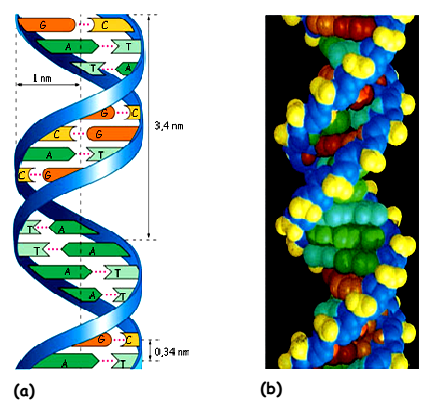
\includegraphics[scale=0.8]{DNA.png}
\caption{Struktura DNA: a) 2D model, b) 3D model}
\label{fig:DNA}
\end{figure}

\begin{figure}[h!t]
\centering 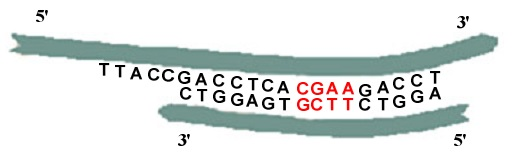
\includegraphics[scale=0.8]{hybrid.jpg}
\caption{Hibridizacija}
\label{fig:hybrid}
\end{figure}

\begin{figure}[h!t]
\centering 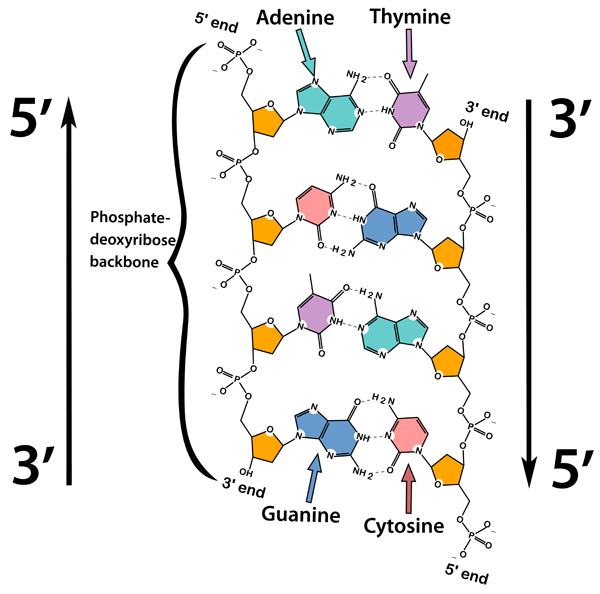
\includegraphics[scale=1]{antipar.jpg}
\caption{Antiparalelnost DNA}
\label{fig:antipar}
\end{figure} 


\begin{figure}[h!t]
\centering 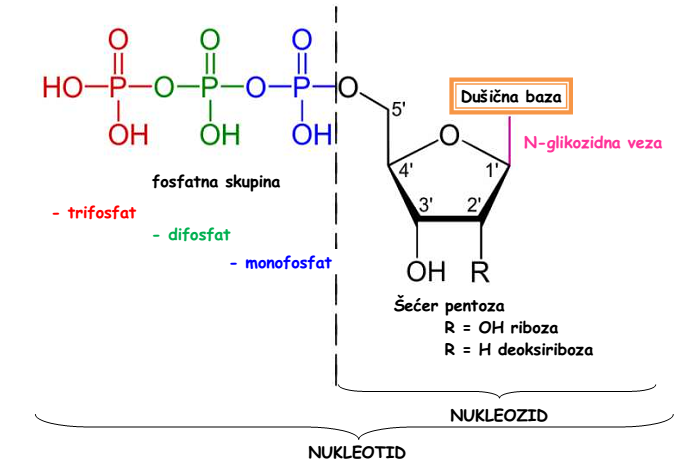
\includegraphics[scale=0.5]{Nukleotid.png}
\caption{Nukleotid}
\label{fig:Nukleotid}
\end{figure} 

\newpage
\begin{comment}
\section{Reprezentacija podataka DNA lancima}
Reprezentacija podataka DNA lancima se vrši na idući način:
\texttt{ 
 \begin{enumerate}
 \item Ulaz: Tekst $T$
 \item Tekst $T$ $\to$ ASCII $T_A$ (Decimalni ili Hex)
 \item ASCII $T_A \to$ 8-bitni binarni prikaz $T_B$ 
 \item Svaka $2$ bita zamijeni pripadnom dušićnom bazom prema \ref{tab:rep}
\end{enumerate}
}
\begin{table}[!ht]
\centering
\begin{tabular}{|c|c|}
\hline 
$\mathbf{x \in \{0,1\}^2}$ & \textbf{Dušićna baza} \\ 
\hline 
00 & A \\ 
\hline 
01 & C \\ 
\hline 
10 & G \\ 
\hline 
11 & T \\ 
\hline 
\end{tabular}
\caption{Reprezentacija uređenog para bitova sa dušićnim bazama}
\label{tab:rep}
\end{table} 
\begin{exa}
Reprezentirajmo "DNA" sa DNA lancem:
\begin{table}[!ht]
\centering
\begin{tabular}{|c|c|c|c|}
\hline 
Tekst & ASCII kod & Binarni prikaz & DNA prikaz \\ 
\hline 
D & 44 & 01 00 01 00& CACA \\ 
\hline 
N & 4E & 01 00 11 10 & CATG \\ 
\hline 
A & 41 & 01 00 00 01 & CAAC \\ 
\hline 
\end{tabular} 
\caption{Reprezentacija riječi "DNA" DNA lancem }
\label{tab:prim}
\end{table}\\
Iz \ref{tab:prim} slijedi:
$"DNA"=(CACACATGCAAC)_{DNA}$
\end{exa}
Naravno, vidimo da bi ovakvu "šifru" bilo iznimno lako probiti pa reprezentaciju podataka nećemo razmatrati kao potencijalni kriptosustav jer bi njegova sigurnost bila izuzetno mala.
\end{comment}
\section{Osnove kriptografije}
\label{sec:kripto}
Kriptografija je znanstvena disciplina koja proučava metode koje u nesigurnom komunikacijskom kanalu  čuvaju integritet i sigurnost podataka i poruka te skrivaju njihov sadržaj od treće osobe, a tako da dane poruke može pročitati samo onaj kome su namijenjene. Razmatrat ćemo komunikaciju između dvoje sudionika: \textit{pošiljatelja (Alice)} i \textit{primatelja (Bob)}. Alice želi preko nesigurnog komunikacijskog kanala poslati poruku, tako da  treća osoba (Oscar ili Eva) ne može saznati sadržaj poruke. Poruku zovemo \textit{otvoreni tekst}. Kako bi sakrila sadržaj poruke, Alice transformira otvoreni tekst uporabom \textit{ključa}. Cijeli postupak transformacije sa ključem nazivamo \textit{šifriranje}, a rezultat šifriranja \textit{šifrat}. Alice šalje Bobu šifrat preko nesigurnog komunikacijskog kanala. Treća osoba pokuašava ukrasti šifrat te saznati njegov sadržaj, no ako je Alice koristila "dobro" šifriranje, treća osoba to neće bit u mogućnosti napraviti. Kada poruka dođe do Boba, on će, u slučaju da ima odgovarajući ključ, šifrat ponovno transformirati u otvoreni tekst, što zovemo \textit{dešifriranjem}. \textit{Kriptoanaliza (dekriptiranje)} je znanstvena disciplina koja proučava metode za čitanje skrivenih poruka bez poznavanja ključa. Kriptologija je znanstvena diciplina koja objedinjuje i kriptografiju i kriptoanalizu. Često za šifriranje odnosno dešifriranje koristimo određene postupke - \textit{kriptografske algoritme (šifre)}. Ti postupci su zapravo određene funkcije - funkcija \textit{enkripcije} općenito otvorenom tekstu (njegovim sastavnim jedinicama) pridružuje osnovne sastavnice šifrata, dok funkcija \textit{dekripcije} opet sastavnim jedinicama šifrata pridružuje sastavne jedinice otvorenog teksta. \textit{Prostor ključeva} je skup čiji su elementi svi mogući ključevi. \textit{Kriptosustav} objedinjuje kriptografski algoritam,   šifrate, ključeve te sve moguće otvorene tekstove.
Sada navodimo formalnu definiciju kriptosustava:
\begin{defn}
Kriptosustav je uređena petorka $(\mathcal{P}, \mathcal{C}, \mathcal{K}, \mathcal{E}, \mathcal{D})$ gdje su redom:
\begin{itemize}
	\item $\mathcal{P}$ konačan skup čije elemente nazivamo \textit{simbolima otvorenog teksta}
	\item $\mathcal{C}$ konačan skup čije elemente nazivamo \textit{simbolima šifrata}
	\item $\mathcal{K}$ je konačan skup čije elemente nazivamo \textit{ključevi}
	\item $\mathcal{E}=\{e :e \text{  je funkcija definirana sa e }:\mathcal{P} \to \mathcal{C} \}$ i $\mathcal{D}=\{d: d\text{ je funkcija definirana sa } d: \mathcal{C} \to \mathcal{P}\}$ su skupovi funkcija za koje vrijedi:
	\[(\forall K \in \mathcal{K})(\exists e_K \in \mathcal{E})(\exists d_K \in \mathcal{D}) : d_K(e_K(x))=x, \forall x \in \mathcal{P} \]
	
\end{itemize}
\end{defn}
\begin{rem}
U primjeni se često radi jednostavnosti kaže da je $\mathcal{P}$ konačan skup osnovnih elemenata otvorenog teksta, a $\mathcal{C}$ skup osnovnih elemenata šifrata. U zadnjoj točki definicije, radi jednostavnosti, navodi da je $x$ otvoreni tekst (odnosno $x \in \mathcal{P}^k$, za neki $k \in \N$). Naravno, to je zbog toga što se prirodno može uvesti "proširenje" funkcije $e_K$ i to na sljedeći način: \\ 
za $\vec{x}=(x_1,...,x_n) \in \mathcal{P}^n$ definira se da je \[e_K(\vec{x})=e_K(x_1)e_K(x_2)...e_K(x_n)\]
Analogno bi se "proširila" funkcija $d_K$. 
\end{rem}
Od načina (tipa operacija) šifriranja razlikujemo \textit{supstitucijske šifre} (svaki element otvorenog teksta se zamijenjuje nekim drugim tekstom, npr. "DNA" $\to$ "GRD"), \textit{transpozicijske šifre} u kojoj se permutiraju slova otvorenog teksta (npr. "DNA" $\to$ "NDA"). Postoje i kriptosustavi koji koriste i jednu i drugu metodu. Otvoreni tekst možemo pak podijeliti na blokove pa razlikujemo \textit{blokovne šifre} i  \textit{protočne šifre}	gdje šifriramo element po element otvorenog teksta. Prema javnosti ključeva razlikuejmo \textit{simetrične kriptosustave} i \textit{kriptosustave s javnim ključem}. U simetričnim kriptosustavima se ključ za dešifriranje može saznati iz ključa za šifriranje, pa je taj ključ \textit{tajan}, zbog čega ove kriptosustave nazivamo i \textit{kriptosustavi s tajnim ključem}. U drugom navedenom postoje dva ključa i ključ za dešifriranje se ne može izvesti iz ključa za šifriranje u nekom razumnom vremenu. U daljnjim razmatranjima pretpostavljat ćemo takozvano Kerckhoffsovo načelo:
\begin{center}
	\textit{Kriptosustav bi trebao biti siguran čak i ako se sve zna o njemu osim ključa.}
\end{center}
Pa ćemo pretpostaviti da napadač na kriptosustav zna koji alat za šifriranje koristimo, posjeduje šifrat i njemu odgovarajući otvoreni tekst, pretpostavljamo da ima mogućnost odabira otvorenog teksta i njemu pripadajućeg šifrata pa čak i da ima alat za dešifriranje na temelju kojeg iz danog šifrata može dobiti otvoreni tekst (cilj mu je saznati ključ za dešifriranje). Prirodno pitanje koje se postavlja jest: postoji li savršeno sigurni kriptosustav. O pojmu savšrene sigurnosti govorio je kriptograf Claude Shannon, prema njegovoj definiciji je kriptosustav savršeno siguran ukoliko šifrat nedaje nikakvu informaciju o otvorenom tekstu, preciznije: neka je $x$ fiksirani otvoreni tekst iz prostora otvorenih tekstova koji se pojavljuje s vjerojatnošću $\mathbb{P}(x)$, tada je uvjetna vjerojatnost $\mathbb{P}(x|y)$ da je $x$ otvoreni tekst, ako znamo da je $y$ šifrat, jednaka $\mathbb{P}(x)$, odnosno:
\[\mathbb{P}(x|y)=\mathbb{P}(x), \quad \forall	 y \in \mathcal{C}\] 
gdje je $\mathcal{C}$ prostor svih šifrata.\\ 
Kada se govori o savršeno sigurnom kriptografskom sustavu, često nailazimo na pojam jednostruke bilježnice (\textit{eng. \textbf{o}ne-\textbf{t}ime \textbf{p}ad}). Kriptosustavi koji koriste koncept jednostruke bilježnice zaprvo koriste kriptografske ključeve koji vrlo često budu izabrani na slučajan način te se upotrebljavaju kako bi se šifrirao točno jedan otvoreni tekst, a nakon toga se više ne koriste. Takav koncept se upravo koristi u DNA kriptografiji, čiju ćemo primjenu vidjeti u poglvalju \ref{sec:EDDNA}.
Više o kriptografiji se može naći u \cite{duje}
\section{DES kriptosustav}	
\subsection{Kratki prgled DES kriptosustava}
"Krajem 60-tih i početkom 70-tih godina 20. stoljeća, razvojem financijskih transakcija, kriptografija postaje zanimljiva sve većem broju potencijalnih korisnika. Dotad je glavna primjena kriptografije bila u vojne i diplomatske svrhe, pa je bilo normalno da svaka država (ili čak svaka zainteresirana državna organizacija) koristi svoju šifru za koju je vjerovala da je najbolja. No, tada se pojavila potreba za šifrom koju će moći koristiti korisnici širom svijeta, i u koju će svi oni moći imati povjerenje - dakle, pojavila se potreba uvođenja standarda u kriptografiji.\\
Godine 1972. američki National Bureau of Standards (NBS) inicirao je program za zaštitu računalnih i komunikacijskih podataka. Jedan je od ciljeva bio razvijanje jednog standardnog kriptosustava. Godine 1973. NSB je raspisao javni natječaj za takav kriptosustav. Taj kriptosustav je trebao zadovoljiti sljedeće uvjete:
\begin{itemize}
\item visoki stupanj sigurnosti
\item potpuna specifikacija i lako razumijevanje algoritma
\item sigurnost leži u ključu, a ne u tajnosti algoritma
\item dostupnost svim korisnicima
\item prilagodljivost uporabi u različitim primjenama
\item ekonomičnost implementacije u elektoničkim uređajima
\item efikasnost
\item mogućnost provjere
\item mogućnost izvoza (zbog američkih zakona)
\end{itemize}

Na tom natječaju niti jedan prijedlog nije zadovoljavao sve ove zahtjeve. Međutim, na ponovljeni natječaj iduće godine pristigao je prijedlog algoritma koji je razvio IBM-ov tim kriptografa. Algoritam je zasnovan na tzv. Feistelovoj šifri. Gotovo svi simetrični blokovni algoritmi koji su danas u uporabi koriste ideju koju je uveo Horst Feistel 1973. godine. Jedna od glavnih ideja je alternirana uporaba supstitucija i transpozicija kroz više iteracija (tzv. rundi).
Predloženi algoritam je nakon nekih preinaka, u kojima je sudjelovala i National Security Agency (NSA), prihvaćen kao standard 1976. godine i dobio je ime Data Encryption Standard (DES)."\footnote{\cite[s. ~?]{duje}}\\
Pogledajmo sada kako se kriptira DES algoritmom:
Pretpostavljamo da je duljina otvorenog teksta $x$ kojeg DES šifrira duljine 64 bita. DES koristi ključ $K=k_1...k_{56}$ duljine 56 bita.
Neka je $x=x_1...x_{64}$ otvoreni tekst. Najprije permutiramo $x$ fiksnom \textit{inicijalnom permutacijom} IP te dobivamo $x_0=IP(x)$ - IP $i$-ti bit od $x$ zamijenjuje sa $IP(i)$-tim bitom od $x$. Inicijalna permutacija IP je prikazana na slici \ref{fig:IP}.

\begin{figure}[h!t]
\centering 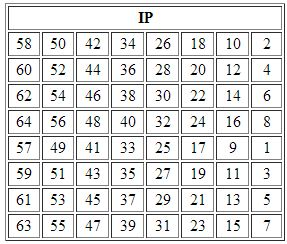
\includegraphics[scale=1]{IP.jpg}
\caption{Inicijalna permutacija}
\label{fig:IP}
\end{figure}

Zatim napišemo $x_0$ u obliku konkatenacije dva \textit{stringa bitova} koji su duljine 32 bita svaki: $x_0=L_0R_0$ 
Nakon toga računamo $L_i$ i $R_i$, gdje je:
\[L_i=R_{i-1}\]
\[R_i=L_{i-1} \oplus f(R_{i-1}, K_i)\]
Gdje su $K_1,...,K_{16}$ \textit{riječi bitova} duljine 48, dobiveni permutiranjem nekih bitova iz $K$. $\oplus$ je operacija \textit{ekskluzivno ili} opisana slikom \ref{fig:XOR}

\begin{figure}[h]
\centering 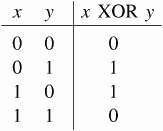
\includegraphics[scale=0.8]{XOR.png}
\caption{Operacija \textit{ekskluzivno ili}}
\label{fig:XOR}
\end{figure}
Sada ćemo opisati dijelovanje funkcije $f:\{0,1\}^{32} \times \{0,1\}^{48} \to \{0,1\}^{32}$. Pretpostavimo da su argumenti funkcije riječ $A$ duljine 32 i $J$ duljine 48.
Prvo niz $A$ proširimo do riječi bitova duljine 48 primjenjujući funkciju $E:\{0,1\}^{32} \to \{0,1\}^{48}$ danu slikom \ref{fig:fjaE} koja $i$-tom bitu, pridruži $E(i)$-ti bit riječi $A$ koji se nalazi na $i$-tom mjestu tablice čitajući s lijeva na desno. Očigledno je da se 16 bitova riječi $A$ "ponavlja".
\begin{figure}[h]
\centering 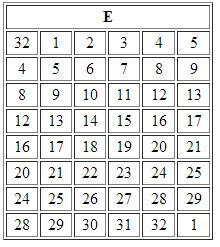
\includegraphics[scale=1]{E.jpg}
\caption{Preslikavanje \textit{E}}
\label{fig:fjaE}
\end{figure}
Uzmemo da je $B=E(A)\oplus J$ te prikažemo $B$ kao konkatenaciju osam riječi sastavljenih od bitova koje su duljine šest, odnosno: $B=B_0B_1B_2B_3B_4B_5B_6B_7B_8$. U sljedećem koraku algoritma koristimo $S-kutije$ (\textit{supstitucijske kutije}) $S_1, ..., S_8$ (prikazane na slici \ref{fig:sbox}), od kojih je svaki $S_i \in \{0,...,15\}^{4\times 16}$ matrica sa 4 retka i 16 stupaca čiji su elementi iz skupa $\{0,...,15\}$. Neka je svaki $B_j=b_1^{(j)}...b_6^{(j)}$. Sada računamo $S_j(B_j)$ prema sljedećem opisu:\\$r_j=b_1^{(j)}b_6^{(j)}$ binarni zapis $r_j$-tog retka od $S_j$, a $c_j=b_2^{(j)}b_3^{(j)}b_4^{(j)}b_5^{(j)}$ binarni zapis $c_j$-tog stupca matrice $S_j$. Definiramo: $C_j=S_j(B_j)=S_j(r_j, c_j), j=1,...,8$ zapisano kao riječ (broj) sastavljenu od 4 bita. Sada riječ $C=C_1C_2C_3C_4C_5C_6C_7C_8$ sastavljenu od 32 bita permutiramo pomoću fiksne \textit{završne permutacije} $P$ prikazane na slici \ref{fig:permP}. U konačnici, vrijedi da je $f(A,J)=P(C)$.	
\begin{figure}[h]
\centering 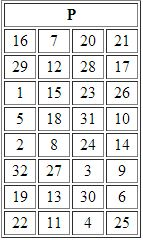
\includegraphics[scale=1]{P.jpg}
\caption{Završna permutacija}
\label{fig:permP}
\end{figure}

Sada opisujemo računanje $K_1,...,K_{16}$ iz $K=k_1...k_{64}$. Bitovi, čiji je indeks $l*8, l=1,...,8$ služe za testiranje pariteta, definirani su tako da svakih osam bitova (jedan bajt), čitajući s lijeva na desno, sadrži neparan broj jedinica. Navedene (paritetne) bitove ignoriramo kod računanja tablice ključeva, a preostale bitove permutiramo  pomoću fiksne permutacije $PC1$ dane slikom \ref{fig:PC1}. Neka je sada $PC1(K)=C_0D_0$, tako da je $d(C_0)=d(D_0)=28$. Sada za svaki $i \in \{1,...,16\}$ računamo:
\[C_i=\begin{cases}^1\overleftarrow{C_{i-1}} &\mbox{ako } i=1,2,9,16 \\  ^2\overleftarrow{C_{i-1}} &\mbox{inače } \end{cases}\]
\[D_i=\begin{cases}^1\overleftarrow{D_{i-1}} &\mbox{ako } i=1,2,9,16 \\  ^2\overleftarrow{D_{i-1}} &\mbox{inače } \end{cases}\]
\[K_i=PC2(C_iD_i)\]
Gdje je $PC2$ fiksna permutacija opisana slikom \ref{fig:PC2}, a operator $^j\overleftarrow{A}$ predstavlja ciklički pomak ulijevo za  $j$ mjesta nad riječi $A$ sasatavljenoj od bitova.
\begin{figure}[h]
\centering 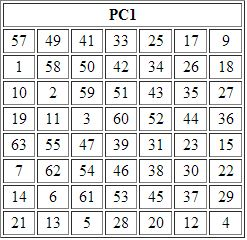
\includegraphics[scale=0.8]{PC1.jpg}
\caption{Fiksna permutacija $PC1$}
\label{fig:PC1}
\end{figure}

\begin{figure}[h]
\centering 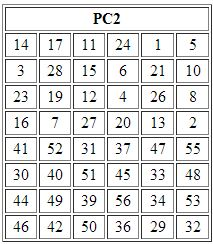
\includegraphics[scale=0.8]{PC2.jpg}
\caption{Fiksna permutacija $PC2$}
\label{fig:PC2}
\end{figure}

Nakon tog cijelog postupka primjenimo \textit{inverznu permutaciju} $IP^{-1}$ na $R_{16}L_{16}$, a onda je šifrat $y$ dan sa:
\[y=IP^{-1}(R_{16}L_{16})\]
Primjetimo da smo sa inverznom permutacijom dijelovali na riječ $R_{16}L_{16}$,a ne $L_{16}$ i $R_{16}$ (obrnuti poredak). Permutacija $IP^{-1}$ je prikazana slikom \ref{fig:invIP}.
Postupak za deđifriranje je analogan:\\
Krećemo od šifrata $y$: na njega najprije primjenimo permutaciju IP sa slike \ref{fig:IP}, $y_0=IP(y)=IP(IP^{-1}(R_{16}L_{16}))=R_{16}L{16}$.  A sada imamo:
\[R_{15}=L_{16}\]
A iz 
\[R_{16}=L_{15} \oplus f(R_{15}, K_{16})\]
Slijedi
\[L_{15}=R_{16} \oplus f(R_{15}, K_{16})\]
Općenito, za sve $i=1,...,16$ dobivamo da vrijedi:
\[R_{16-i}=L_{16-i+1}\]
\[L_{16-i}=R_{16-i+1} \oplus f(R_{16-i}, K_{16-i+1})\]
Iz čega dobivamo niz $R_{14}L_{14},R_{13}L_{13},...R_{0}L_{0}$. A zatim zamjenom poretka od $R_{0}L_{0}$ i primjenom na to $IP^{-1}$ dobivamo:
$IP^{-1}(L_0R_0)=IP^{-1}(IP(x))=x$
Pa smo dobili traženi otvoreni tekst. Primjer šifriranja otvorenog teksta pomoću DES kriptosustava može se naći na \cite{DESexa}. O implementaciji DES-a na DNA računalu se može naći u \cite{DESDNA}, u ovom radu, fokusirat ćemo se više na provaljivanje DES kriptosustava opisanom u idućem poglavlju.
\begin{figure}[h]
\centering 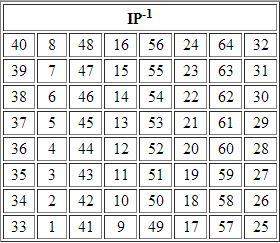
\includegraphics[scale=0.7]{invIP.jpg}
\caption{Inverzna permutacija $IP^{-1}$}
\label{fig:invIP}
\end{figure}

\begin{figure}[h]
\centering 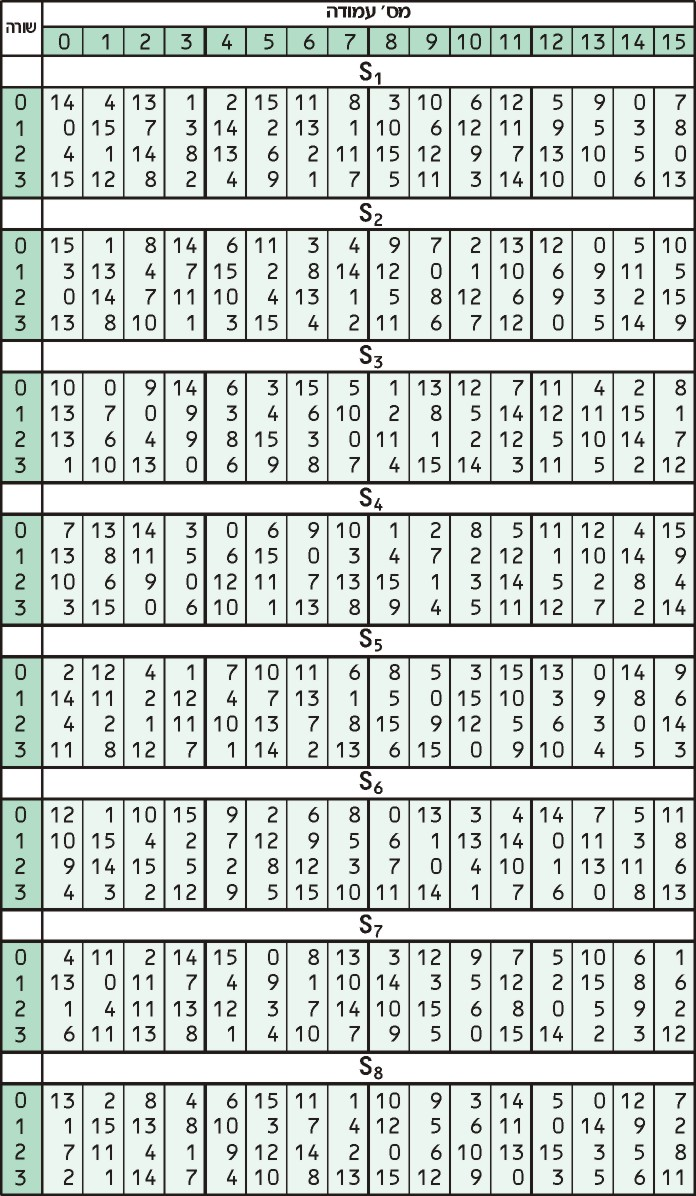
\includegraphics[scale=0.52]{S-box.jpg}
\caption{$S$-kutije}
\label{fig:sbox}
\end{figure}
 \newpage
\subsection{Provaljivanje DES-a DNA izračunavanjem}
\subsubsection{Uvod i oznake}
U poglavlju \ref{sec:DNAizr} smo naveli opisnu definiciju DNA računala koju je predložio Leonard Adleman, a u poglavlju \ref{sec:DNA} su navedene osnovne činjenice i neke od biokemijskih operacija koje se koriste u genetičkom inženjeringu. U ovom poglavlju ćemo koristiti operacije navedene upravo u \ref{sec:DNA} te nećemo te operacije striktno definirati u definiciji navedenoj u poglavlju \ref{sec:DNAizr} premda bi se mogle. Naime, ta definicija je služila kao osnovni matematički koncept kojeg je predložio Adleman, a koji se kasnije postupno proširivao. Kako su se proširivala istraživanja o DNA i genetičkom inženjeringu, tako bi se i dana definicija mogla izmjenjivati. Opisat ćemo oznake i biokemijske operacije koje ćemo koristiti.
Neka je $x$ proizvoljna riječ alfabeta $\Sigma =\{\mathtt{A,C,G,T}\}$. Biološki gledano, $x$ nije još DNA lanac jer nema orijentaciju. Nadalje, uvodimo Watson-Crickov komplement (biološki komplement u poglavlju \ref{sec:DNAizr}). To je preslikavanje opisano sa ($\mathtt{A \to T, T \to A, G \to C, C \to W}$). Watson-Crickov komplement označavat ćemo sa $\overline{x}$. Sa $x^R$ ćemo označavati riječ koja je sastavljena od istih simbola kao i riječ $x$ samo u obrnutom poretku. Sa $\mathtt{\uparrow} x$ ćemo označavati  jednolančani DNA čija je orijentacija $\mathtt{5' \to 3'}$, a sastavljena  je od niza simbola od kojih se sastoji $x$. Sa $\downarrow x$ ćemo označavati lanac orijentacije $3'->5'$ sa nizom simbola koji čine Watskon-Crickov komplement niza $x$. U konačnici, sa $\mathtt{\updownarrow x}$ označavamo dvolančanu strukturu nastalu spajanjem $\mathtt{\uparrow x}$ i $\mathtt{\downarrow x}$. Kako bi svatili sve oznake napravit ćemo jedan primjer:
\begin{exa}
Neka je $x=\mathtt{TGCCGCAG}$ riječ alfabeta $\Sigma=\mathtt{\{A,C,G,T\}}$, tada je:
\[\overline{x}= \mathtt{ACGGCGTC}\]
\[x^R=\mathtt{GACGCCGT}\]
\[\uparrow x=\mathtt{5'-TGCCGCAG-3'}\]
\[\downarrow x=\mathtt{3'-ACGGCGTC-5'}=	\uparrow \overline{x}^R\]
\[\updownarrow x=\mathtt{{5'-TGCCGCAG-3' \atop 3'-ACGGCGTC-5'}}\]
\end{exa}
\subsubsection{Reprezentacija riječi sastavljenih od alfabeta $\{0,1\}$}
\label{subsub:repBit}
Neka je $x=x_1x_2...x_n$ proizvoljna riječ alfabeta $\{0,1\}$ duljine $n$. Ideja je svakom bitu pridružiti jedinstveni $30$-mer -- oligonukleotida duljine $30$. Kasnije ćemo vidjeti da osim jedinstvenog $30$-mera svaki bit mora imati jedinstvenu reprezentaciju.
\begin{enumerate}
\item $B_i (0)$ označava oligonukleotidu koja reprezentira da je $i$-ti bit riječi $x$ jednak 0
\item $B_i(1)$ označava oligonukleotidu koja reprezentira da je $i$-ti bit riječi $x$ jednak 1
\item Za $i \in \{0,1...,n\}$ neka je $S_i$ $30$-mer koji označava separator između susjednih bitova
\end{enumerate}   
U konačnici, DNA lanac koji reprezentira binarni string $x$ je:
\[\updownarrow S_0 B_1(x_1)S_1B_2(x_2)S_2...S_{n-1}B_n(x_n)S_n\]
Svi $B_i$-ovi i $S_i$-ovi su međusobno različiti, , štoviše kasnije ćemo vidjeti da će biti nužno da svaka dva bita nemaju zajedničke podriječi čija je duljina veća ili jednaka $15$. To se može postići tako da riječi $B_i(b)$ i $S_i$ budu izabrane na slučajan način, budući da zajednička podriječ dvije slučajno izabrane riječi ima tendenciju biti što kraća. Upravo smo iz toga razloga uzeli $30$-mere kao riječi koje će predstavljati bitove, s druge strane biokemijskim reakcijama u laboratoriju će trebati duže da se odviju nad $30$-merima nego nad nekim kraćim oligonukleotidama. Adleman je tako za svoj eksperiment opisan u \cite{Adleman} koristio $20$-mere, no njegov problem je imao manje podataka koje je morao reprezentirati. Uočimo da će svaki bit biti reprezenitran sa dva stringa iz skupa $\mathbb{Y}=\{(y_1,...,y_15): y_i \in \mathtt{\{A,C,G,T\}\}}$, pa je vjerojatnost da dvije riječi imaju istu podriječ duljine $15$ jednaka $p=\left(\frac{1}{4^{15}}\right)^2=\frac{1}{1152921504606846976}\approx 8.6736 \cdot 10^{-19}\approx 0$. Stringovi $S_0$ i $S_n$ će u replikaciji s PCR-om služiti kao početnice. Uvodimo još oznaku $R_i(x)$ koja će označavati sljedeću riječ:
\[R_i(x)=B_i(x_1)S_iB_{i+1}(x_2)S_{i+1}...S_{i+n-2}B_{i+n-1}(x_n)S_{i+n-1}\]
\subsubsection{Opće biokemijske operacije}
\paragraph{Hibridizacija (taljenje i hlađenje)}
Postoje dvije biokemijske reakcije, čiji je rezultat isti, a kojima se postiže spajanje dva komplementarna lanca. Jedna se zove hibridizacija, a druga je metoda taljenja i hlađenja. Osnovni rezultat tih operacija je prikazan donjom jednadžbom:
\[\mathtt{\uparrow x + \downarrow x=\updownarrow x}\]
Ona opisuje operaciju spajanja dva jednolančana DNA lanca u jedan dvolančani. Pod hibridizacijom (ili postupkom taljenja i hlađenja) je moguća i sljedeća reakcija:
\[\mathtt{\uparrow xy + \downarrow yz = \uparrow x \updownarrow y \downarrow z}\].
\paragraph{Ekstrakcija ili izdvajanje}
Drugu operaciju koju ćemo koristiti naziva se ekstrakcija. Služi za  izdvajanje onih DNA lanaca koji kao podriječ sadrže riječ $\mathtt{x}$. To se biokemijski ostvaruje na sljedeći način:\\
U epruvetu se dodaje dovoljan broj kopija od $\mathtt{\downarrow x}$ koje se nalaze na određenoj površini premazanoj gelom koji u sebi sadržio biotin-streptavidin (na primjer na staklu ili Petrijevoj zdjelici) te djeluju poput magneta. Zatim se postupkom hibridizacije događa na primjer:
\begin{equation}
\label{eq:DNAExt}
\mathtt{\uparrow vxw + \downarrow x = \uparrow v \updownarrow x \uparrow w}
\end{equation}
Nakon toga se na tom gelu nalaze sve riječi koje poprimaju oblik sličan onome s desne strane jednakosti u jednadžbi \ref{eq:DNAExt} (no nalaze se i oligonukleotide $\mathtt{\downarrow x}$ jer neće sve biti iskorištene -- stavlja se veći broj kopija od potrebnog). Naime osim spajanja koje je prikazano u \ref{eq:DNAExt} moguća su i razna spajanja različitoga oblika (na primjer gdje se oligonukleotida $\mathtt{\uparrow x}$ može biti vezana na početku nekog DNA lanca koji poprima dvolančanu strukturu). U slučaju kad će to biti potrebno istaknuti, na ovu operaciju ćemo se referencirati kao na ekstrakciju koja koristi niz $\mathtt{\downarrow x}$. Kasnije se $\mathtt{\uparrow v \updownarrow x \uparrow w}$ izdvaja pomoću tehnike koja se zove gel elektroforeza, a nakon toga se $\mathtt{\downarrow x}$ odvaja od orginalnih lanaca pomoću enzima DNA helikaze. U našoj primjeni, mi ćemo tu operaciju označavati sa:
\[Extract(T, x_i=1)\]
gdje je $T$ proizvoljna epruveta koja sadrži DNA lance. Ovom operacijom izdvajamo sve one DNA lance koji kao podriječ sadrže $B_i(1)$ (na $i$-tom mjestu binarne riječi nalazi se 1). Naravno osim jednostrukog bita, možemo izdvojiti cijele podriječi, na primjer:
\[Extract(T, x_ix_{i+1}=01)\] 
će izdovjiti sve one binarne riječi koje na $i$-tom i $i+1$-om mjestu imaju redom 0 i 1, a za to će se koristiti DNA lanac $R_i(01)=B_i(0)S_{i}B_{i+1}(1)S_{i+1}$. Uočimo da je to zapravo operacija:
\[Extract(T, x_i=0 \wedge x_{i+1}=1)\]
pa smo napravili "i" operaciju -- ipak to je moguće napraviti samo kad se radi o sujsednim bitovima -- inače, moramo napraviti dvije uzastopne operacije izdvajanja. Na gel kojim premazujemo staklenu površniu osim premaza streptavidin-biodina koji sadrži na primjer sekvencu $R_i(101)$, možemo na istu staklenu površinu i koristiti premaz streptavidin-biodina koji sadrži niz $R_i(001)$. Time će se izvršiti operacija:
\[Extract(T, x_ix_{i+1}x_{i+2}=101 \vee x_ix_{i+1}x_{i+2}=001)\] 
Iz tehničkih, biokemijskih, razloga moguće je samo izvoditi ovakvu simultanu "ili" operaciju kada su binarne riječi koje su argumenti od $R_i$ jednake duljine.
\paragraph{Replikacija} Za razliku od običnog proširivanja opisanog u poglavlju \ref{sec:DNAizr} ovdje ćemo koristiti biokemijsku operaciju replikacije pomoću polimerazne lančane reakcije (PCR - \textbf{p}olymerase \textbf{c}hain \textbf{r}eaction). Da bi PCR mogao djelovati, moraju se zadovoljiti sljedeći uvjeti:
\begin{itemize}
\item svaki lanac mora biti oblika $\mathtt{\updownarrow aBc}$, gdje su $\mathtt{a}$ i $\mathtt{c}$ fiksne riječi, a $\mathtt{B}$ proizvoljna
\item $\mathtt{a}$ i $\mathtt{c}$ se ne smiju pojaviti kao podriječi od $\mathtt{B}$
\end{itemize}
Ako prvi uvjet nije ispunjen, to znači da u epruveti nema takvih riječi. Drugi uvijet će se osigurati duljinom DNA oligonukleotida tako da će biti moguće kreirati točno takve lance -- $\mathtt{a}$ i $\mathtt{b}$ će u riješavanju našega problema biti takve duljine da će njihova vjerojatnost pojavljivanja u $\mathtt{B}$ biti jednaka 0, a tose omogućuje i reprezentacijom bitova opisanoj u \ref{subsub:repBit}. Podriječi $\mathtt{a}$ i $\mathtt{b}$ zovemo početnice (\textit{eng. primers}). Ova operacija omogućuje sintetičku proizvodnju kopije proizvoljne riječi $B$ (uočimo da je efekt jako sličan onom efektu operacije proširivanja opisane u poglavlju \ref{sec:DNAizr}).

\paragraph{Označavanje} Na određeni DNA lanac, dodajemo novu oligonukleotidu $\mathtt{z}$, a postpuak je opisan sljedećim koracima:\\
Uvjet svaki lanac je oblika $\mathtt{\uparrow Xy}$, gdje je $\mathtt{X}$ proizvoljan, a $\mathtt{y}$ fiksiran:
\begin{equation}
\label{eq:Tag1}
\mathtt{\uparrow Xy + \downarrow yz=\uparrow X \updownarrow y \downarrow z}
\end{equation}
Zatim se dodaje enzim DNA polimeraza koji će konvertirati paricajlni dvolančani lanac iz desne strane jednakosti jednadžbe \ref{eq:Tag1} u potpuni. Najprije se "čitaju" jednolančane porcije s desne strane jednakosti od \ref{eq:Tag1} i kreiraju njihovi Watson-Ckrickovi komplementi, za svaku nukleotidu u jednom trenutku. Odnosno događaju se pojedinačno sljedeće reakcije:
\begin{equation}
\label{eq:Tag2}
\mathtt{\uparrow X \updownarrow y \downarrow z + \downarrow X = \updownarrow Xy \downarrow z}
\end{equation}
\begin{equation}
\label{eq:Tag3}
\mathtt{\updownarrow Xy \downarrow z + \uparrow z = \updownarrow Xyz}
\end{equation}
Zatim se opet pomoću DNA helikaze dobiva $\mathtt{\uparrow Xyz}$.

\subsubsection{Plan napada na DES kriptosustav i algoritam}
Označimo s $DES(M,k)$ šifrat dobiven enkripcijom otvorenog teksta $M$ koristeći ključ $k$ u DES kriptosustavu. U poglavlju \ref{sec:kripto} smo napomenuli da napadač na dani kriptosustav obično ima odabrani otvoreni tekst i njemu pripadajući šifrat. U tu svrhu pretpostavit ćemo da je parametar $M_0$ neki fiksan $64$-bitni otvoreni tekst, a $k$ ključ kojeg pokušavamo naći. Poznato je da otvorenom tekstu $M_0$ pripada šifrat $E_0$. Tada za dani $M_0$ uvodimo funkciju $f:\{0,1\}^{56} \to \{0,1\}^{64}$ koja za neki ključ $k$ proizvoljan, tekstu $M_0$ pridružuje šifrat $DES(M_0,k)$, odnosno $f(K)=DES(M_0,k)$. Jedno svojstvo DES kriptosustava jest da će ključ $k_0$ biti upravo jedinstven. Naša je zadaća naći $k_0$ takav da je $f(k_0)=E_0$, odnosno naći inverz funkcije $f$ ako su nam poznati otvoreni tekst i njegov pripadni šifrat. Ono što ćemo napraviti jest konsturiranje svih parova $[k, f(k)]$ za svih $2^{56}$ mogućih ključeva. Pošto su permutacije u $DES$ kriptosustavu fiksirane, a neke od njih samo skraćuju ili nadodaju još bitova na točno određeni način, za naše primjene te permutacijske kutije ne igraju značajnu ulogu i mogu biti ignorirane. Naime, nema potrebe da  fizički permutiramo bitove u DNA lancima, već samo možemo pratiti (na primjer na papiru) bitove DNA lanca koji kodiraju bitove u izračunavanju. Za računanje operacije $\oplus$ i $S$-kutija radimo sljedeće:
Pretpostavimo da želimo izračunati XOR ($\oplus$) $i$-tog i $j$-tog bita u epruveti $T$. To ćemo učitniti dodajući vrijednost $x_i \oplus x_j$ na DNA lanac koji reprezentira riječ $x$. Prvi korak u tome je razdvajanje epruvete $T$ na dva riješenja $T_0, T_1$ gdje vrijedi:
$T_0=\{x \in T| x_i \oplus x_j=0 \}$, a $T_0=\{x \in T| x_i \oplus x_j=1 \}$. Definiramo međurješenje na idući način:
\[T^{11}=Extract(T, x_i=1 \vee x_j=1)\]
\[T^{1}=Extract(T^{11}, x_i=0 \vee x_j=0)\]
\[T^{0}=T\backslash T^{1}\]
Jedna $S$-kutija zaravo odgovara preslikavanju: $g: \{0,1\}^6 \to \{0,1\}^4$. Pretpostavimo sada da su bitovi koje želimo preslikati (na koje dijeluje $S$-kutija) počinju na poziciji $i$, a završavaju na poziciji $i+5$, svakom DNA lancu $x$ želimo prilijepiti $4$-bitnu riječ  $g(x)$. To se radi tako da se rješenje $T$ razdvaja na 16 različitih riješenja $T_0,...,T_{15}$ ovisno prema vrijednosti koja se dodjeljuje. Tada ćemo svakom pojedinačnom rješenju $T_j$ nadodati $4$-bitnu riječ $j$. Na primjer, pretpostavimo da funkcija $g$ preslikava $6$-bitne riječi $a$ i $b$ u $0$, i ne postoji riječ $c \in \{(x_1,...,x_6)| x_i \in \{0,1\}\}\backslash \{a,b\}$ takva da je $f(c)=0$. Tada je:
\[T_0 \leftarrow Extract(T, x_i...x_{i+5}=a \vee x_i...x_{i+5}=b)\]
Preostale operacije ekstrakcije se rade na sličan način. Ovo pokazuje da se pojedinačna $S$-kutija može izračunati u $16$ operacija ekstrahiranja i jednako toliko operacija označavanja.	Operacija izdvajanja zahtjeva pripremu od $2^6=64$ različitih premaza biotin-streptavidinom. Ti premazi se pak mogu pripremiti na način kojim će biti kreirana \textit{inicijalna otopina}  za rješavanje problema, a oni će se kasnije koristiti u svih $16$ rundi izračunavanja pa je to dovoljno pripremiti jednom na početku cijelog procesa. Sada kada smo kreirali uvodni dio, krećemo na detaljan opis algoritma za probijanje DES kriptosustava. U tu svrhu pogledajmo donji graf na slici \ref{fig:graf}.
\begin{figure}[h]
\centering 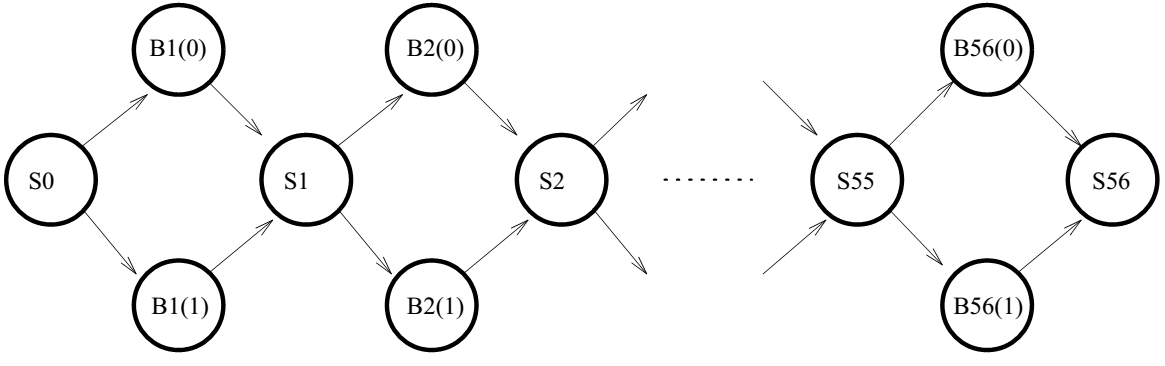
\includegraphics[scale=0.5]{graf.png}
\caption{Inicijalni graf}
\label{fig:graf}
\end{figure}

Svaki put u tom grafu od čvora $S_0$ do čvora $S_{56}$ predstavlja jedan mogući ključ u DES kriptosustavu. Ta percepcija nam treba kako bi jasno shvatili korake algoritma. Važno je naglasiti da ako znamo otvoreni tekst $M_0$ preslikavanje funkcije $f$ koja preslikava ključ u šifrat se zapravo može spremiti u tablicu, a zahvaljujući izuzetnim kapacitetima DNA što se tiče memorije (na primjer 5.5 petabita podataka - što je oko 700 terabajta - je spremljeno u jedan gram DNA)\footnote{\cite{Church}}, $f(k)$ možemo spremiti bez većih problema na DNA, a njen izračun se računa samo na temelju bitova iz $k$ (jer je prva komponenta u $DES(M_0,k)$ konstanta).
\begin{enumerate}
\item Istaknuli smo da za svaki vrh $V$ postoje $15$-meri $V^l$ i $V^r$ takvi da je $V=V^lV^r$ i da ne postoji vrh $U \neq V$ takav da je $U=V^lV^r$ ili $U=V^rV^l$.
\item  Ulaz: Za svaki vrh $v$ kreiraj epruvetu koja sadrži jednolančane DNA $\uparrow V^lV^r$. Za svaki usmjereni vrh $(u,v)$ epruvetu sastavljenu  od jednolančanih DNA $U^rV^l$. Kako bi kreirali potpune dvolančane strukture DNA, kreiraj dvije epruvete od kojih će jedna sadržavati $\uparrow S_0 ^l$, a druga $\downarrow S_{56}^r$
\item Pomiješaj sve epruvete u jednu te započni postupak hibridizacij
\item Ekstrahiraj sve DNA lance koji sadrže riječ $S_0$
\item Ekstrahiraj sve DNA lance koji sadrže riječ $S_{56}$\\
Time smo dobili sljedeće:
\[\updownarrow S_0R_1(k)\]
Gdje je $k \in \{0,1\}^{56}$
\item Izračunaj prijelaze DES sklopovlja za sve ključeve, a pojedini ključ označi rezultatom DES prijelaza. Na primjer, ako prvi prijelaz DES sklopovlja, s obzirom na fiksnu poruku $M_0$ nalaže da se napravi $XOR$ na $2$ i $5$ bitu ključa $k$, tada će ključ nakon izračuna $k_2 \oplus k_5$ biti označen sa $B_{57}(k_2 \oplus k_5)S_{57}$, odnosno dobit ćemo:
\[\updownarrow S_0R_1(k)B_{57}(k_2 \oplus k_5)S_{57}\] 
\item Računamo jedan po jedan prijelaz u DES sklopovlju, a za svaki prijelaz, njegov izlaz dodajmo na kraj svakog DNA lanca, nakon toga svi lanci u riješenju izgledaju kao:
\[\updownarrow S_0R_1(k)R_{57}(I)R_r(DES(M_0,k))\]
Gdje je $I$ riječ bitova koja odgovara izlaznim vrijednostima pojedinih unutarnjih prijelaza u DES sklopovlju. 
\end{enumerate} 
Ovaj algoritam, kada bi se ukupno raspisale sve operacije, koristi 916 koraka i to da se neki koraci izdvajanja izvedu paralelno, a o detaljnoj analizi toga, kao i o daljnjoj optimizaciji algoritma se može naći u \cite{DESbreak}.
\newpage
\section{Enkripcija i dekripcija podataka}
\label{sec:EDDNA}
Funkciju enkripcije i dekripcije ćemo sada opisati:
Neka je $M$ otvoreni tekst koji Alice želi kriptirati i poslati preko nesigurnog komunikacijskog kanala. Alice će najprije pretvoriti $M$ u pripadni $ASCII$ kod, a potom će taj $ASCII$ kod prevesti u binarni otvoreni tekst $M'$. Neka je $m'=d(M')$ duljina binarnog otvorenog teksta $M'$. Označimo s $k_A$ proizvoljan, slučajno izabrani, jednolančani DNA koji će nam poslužiti kao ključ, a koji je duljine $10m'$. Alice kriptira po sljedećem algoritmu:
\begin{enumerate}
	\item $M$ pretvorimo u ASCII $M_A$, a onda $M_A$ u binarni prikaz $M'$ otvorenog teksta $M$
	\item Alice izabire slučajan $d(M')*10$-mer (ssDNA) i koristi ga kao ključ $k_A$
	\item Čitaj $M'$ s lijeva na desno, a čitaj $\overline{k_A}^R$ s  desna na lijevo u blokovima od $10$ dušićnih baza (blokove čitaj s lijeva na desno)
	
	\begin{itemize}
		\item m=0
		\item Dok ne pročitaš sve bitove:
		\begin{itemize}		
			\item Ako je bit jednak $1$\\
		  uzmi dani blok i nadodaj na njega m; \\
			Pošalji blok Bobu\\		  
		   m:=m+1;
			\item Inače (ako je bit jednak $0$)\\
		ignoriraj blok i prijeđi na idući
		\end{itemize}	
	\end{itemize}
\end{enumerate}
Kada Bob primi sve blokove, on dekriptira šifrat po idućem postupku:
\begin{enumerate}
	\item Pročitaj broj zalijepljen na kraj dušićnih baza (označimo ga s $i$) i obriši ga iz bloka
	\item kreiraj Watson-Krickov komplement danog bloka i nađi mjesto gdje se nalazi krećući od indeksa $(d(M')-i-1)\cdot 10$ čitajući blok po blok s desna na lijevo
	\item Svaki blok kojeg Bob nađe zamijenjuje s $1$, a one blokove iz ključa koje Alice nije poslala označi s $0$
	\item Dani binarni string Bob preokreće i nalazi mu ASCII vrijednost, a za ASCII vrijednost mu nađe ekvivalentan otvoreni tekst u prirodnom jeziku 
\end{enumerate}
Slijedi implementacija u programskom jeziku Pythonu.
 \lstset{language=Python,
           basicstyle=\ttfamily,
           keywordstyle=\color{blue}\ttfamily,
           stringstyle=\color{red}\ttfamily,
           commentstyle=\color{green}\ttfamily,
          breaklines=true
          }
\lstinputlisting[language=Python]{enkripcija.py}
Na slici \ref{fig:prim} se može vidjeti primjer enkriptcije i dekripcije pomoću navedene implementacije u Pythonu.
\begin{figure}[h]
\centering 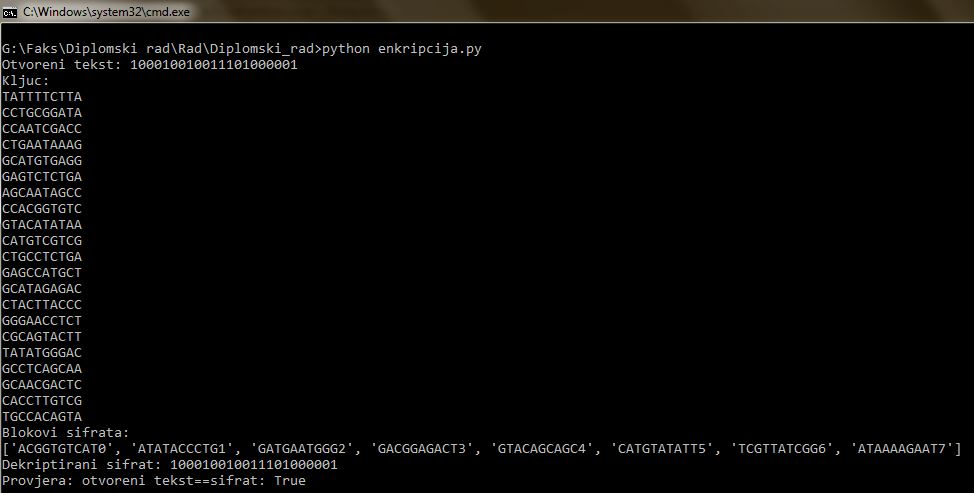
\includegraphics[scale=0.5]{primjer.jpg}
\caption{Primjer enkripcije i dekripcije riječi "DNA"}
\label{fig:prim}
\end{figure}

Implementacija pomoću DNA računala je zapravo jako jednostavna. Za dani otvoreni binarni tekst, Alice samo treba kreirati određene Watson-Crickove komplemente slučajno izabranog ključa, odabrati pripadajuće blokove, te ih poslati Bobu preko nesigurnog komunikacijskog kanala. Bob zatim u epruvetu koja sadrži $\uparrow k_A$, ulije dobivene blokove te pokrene proces hibridizacije. Time dobije određeni DNA lanac koji je na određenim mjestima dolančani, a na određenim jednolančani. Tamo gdje je dvolančani (vidi preko mikroskopa), stavlja bit $1$, a jednolančani bit $0$ te čita dani binarni string s desna na lijevo kreirajući njemu ekvivalentan otvoren tekst u prirodnom jeziku. O različitim načinima kriptiranja pomoću DNA računala može se naći u \cite{borda2011fundamentals}. 
Sigurnost ovog kriptosustava može se povećati uzimanjem ključa koji će biti veće duljine (na primjer da se umjesto za svaki bit uzme $10$-mer, možemo uzeti $40$-mer), i ona ovisi samo o danom ključu (jednokratnoj bilježnici). Nadalje, što je duži tekst koji se šifrira, time će se povećavati i kompleksnost kriptosustava. Tako, na primjer, za kriptiranje riječi $DNA$ čija binarna reprezentacija ima $21$ bit, prostor ključeva sadrži $4^{21\cdot 10}=4^{210}$ različitih ključeva koji mogu šifrirati danu riječ. 
\section{Prednosti i mane DNA računala i DNA kriptografije}
Glavna prednost DNA računala je izrazito veliki kapacitet i gustoća memorije zbog koje se stvari mogu lakše izračunavati i gdje se napadi na kriptosustvae s tehnikom grube sile vrlo lako probijaju. Opet rješavanje nekih $NP$ teških problema se također riješavaju istom tehnikom. Druga prednost je masivna paralelnost DNA računala zbog  toga što se jedna operacija obavlja nad skupom riječi, a ne na samo jednoj riječi (broj procesora varira - to ja kao da broj procesora konstantno varira ovisno o broju podataka u programu). S druge strane DNA računalo može raditi grešku u izračunavanju, odnosno u izvođenju biokemijskih reakcija, o tome kako utjecati na te greške se može naći u \cite{DNAerr}. Daljnja mana je ta što je DNA računalo za sada samo teoretski model izračunavanja jer da bi se moglo konstrukirati i fizički ostvariti trebaju se preći još mnoge tehnološke prepreke kao i fizička ograničenja. DNA računalo dobro računa sa, kako se čini, relativno kompliciranim operacijama (npr. $Replikacija, Ekstrakcija$), no pri izračunavanju jednostavnih operacija kao što je "ekskluzivno ili", potrebno je izvesti $4$ koraka u postupku. Daljnja mana je ta što su operacije na DNA računalu spore u odnosnu na operacije koje se obavljaju na elektromehaničkim računalima. One postaju sporije što je više parova $G$ i $C$ u nekoj dvolančanoj DNA zbog trostrukih kovalentnih veza koje se teže razbijaju i teže uspostavljaju između tih dviju dušićnih baza te što je veća duljina samih DNA lanaca u epruveti. Ipak, kako područja genetike i medicine jako brzo napreduju, postoji mogućnost otkrića kako da se te operacije ubrzaju primjenom nekih katalizatora ili električne energije. 

\newpage
\nocite{*}
\bibliographystyle{abbrv}
\bibliography{borda2011fundamentals,literatura,CNTYan,lipton,DESDNA,Church}
\end{spacing}
\end{document}